\documentclass[letterpaper,journal]{IEEEtran}
% chktex-file 1
% chktex-file 2
% chktex-file 3
% chktex-file 8
% chktex-file 12
% chktex-file 13
% chktex-file 18
% chktex-file 24
% chktex-file 35
% chktex-file 44
\usepackage{amsmath,amsfonts}
\usepackage{algorithmic}
\usepackage{algorithm}
\usepackage{array}
\usepackage[caption=false,font=normalsize,labelfont=sf,textfont=sf]{subfig}
\usepackage{textcomp}
\usepackage{stfloats}
\usepackage{placeins}
\usepackage{url}
\usepackage{verbatim}
\usepackage{adjustbox}
\usepackage{graphicx}
% Images live under latex/img/.  Allow the document to be compiled either from
% the repository root (pdflatex latex/bare_jrnl_new_sample4.tex) or from the
% latex/ directory itself.
\graphicspath{{latex/img/}{img/}}
\usepackage{cite}
\hyphenation{op-tical net-works semi-conduc-tor IEEE-Xplore}
\raggedbottom
\makeatletter
\let\ieeeorigmakecaption\@makecaption
\long\def\@makecaption#1#2{%
	\ifx\@captype\@IEEEtablestring
		\ieeeorigmakecaption{#1}{#2}%
	\else
		\footnotesize
		\setbox\@tempboxa\hbox{#1. #2}%
		\ifdim\wd\@tempboxa >\hsize
			\centerline{\parbox{\hsize}{\centering #1. #2}}%
		\else
			\hbox to\hsize{\hfil\box\@tempboxa\hfil}%
		\fi
	\fi
}
\makeatother
% updated with editorial comments 8/9/2021

\begin{document}

% \title{A Sample Article Using IEEEtran.cls\\ for IEEE Journals and Transactions}
\title{{\fontsize{24pt}{24pt}\selectfont An Open-source and Optimization-based\\ AC/DC Power Flow Model for the Brazilian Interconnected Power System}}

\author{
	\IEEEauthorblockN{Marck Llerena Velasquez\IEEEauthorrefmark{2}, Fernando W. Liederer\IEEEauthorrefmark{2}, Marcos J. Rider\IEEEauthorrefmark{2} and Daniel Dotta\IEEEauthorrefmark{2}}\\
	% \vspace{0.1cm}
	\IEEEauthorblockA{\IEEEauthorrefmark{2}\textit{State University of Campinas (UNICAMP), Campinas, Brazil}} \\
	% \IEEEauthorblockA{\IEEEauthorrefmark{3}\textit{National Laboratory of the Rockies, Colorado, USA}} \\
	\IEEEauthorblockA{marck.llerena-velasquez@nlr.gov, dottad@unicamp.br}
}
% The paper headers
\markboth{}%
{Shell \MakeLowercase{\textit{et al.}}: An Open-source and Optimization-based AC/DC Power Flow Model for the Brazilian Interconnected Power System}

\IEEEpubid{}
% Remember, if you use this you must call \IEEEpubidadjcol in the second
% column for its text to clear the IEEEpubid mark.

\maketitle

\begingroup
\hbadness=10000
\begin{abstract}
	This paper presents an open-source optimization-based integrated AC/DC power flow model for
	the Brazilian Interconnected Power System (BIPS), including detailed representations of
	LCC links and FACTS devices, together with general network control mechanisms. The formulation is a
	nonlinear programming (NLP) problem in which network power-balance equations are enforced as
	exact equalities, while controller equations and operational limits are treated as bounded
	soft constraints through nonnegative slack variables. The model is implemented in Python with
	Pyomo and solved with Ipopt. Validation against Anarede is performed on equivalent and
	large-scale BIPS cases, including two power flow operating snapshots. Results show consistent 
	operating points and robust convergence across the analyzed cases, with expected numerical differences
	from modeling assumptions and solution strategy.
\end{abstract}
\endgroup

\begin{IEEEkeywords}
	AC/DC power flow, BIPS, FACTS, LCC, nonlinear programming, open-source software, optimization, 
	network control components, power flow snapshots.
\end{IEEEkeywords}

\section{Introduction}


Power flow analysis is a fundamental process in power systems operations and planning, since it provides the steady-state voltages,
angles, and power injections used in security assessment and grid studies \cite{ref1}. For many years, this process has been solved mainly
with Newton Raphson and Fast Decoupled methods, which offer good computational performance for conventional AC networks. As modern grids evolve,
however, the modeling scope has expanded beyond the traditional AC setting. The growing integration of FACTS devices and HVDC systems introduces
high nonlinearities, which increases the complexity of the power flow problem \cite{ref2}.
In hybrid AC/DC systems, representations are separated into sequential and integrated formulations. Sequential methods solve AC and DC
subsystems separately and exchange boundary values until convergence \cite{ref3}. This structure reduces matrix size per iteration and is
attractive for large systems, but convergence can be weak in stressed or poorly conditioned cases, especially when many controls and limits
are active \cite{ref4}.

Integrated methods solve AC and DC equations together in a single model, which improves consistency between network states and converter
controls \cite{ref5}. In this same approach, FACTS devices can also be embedded in the power flow equations through steady-state
injection-based representations, enabling their control actions and limits to be handled within the unified network solution \cite{ref6}.
Discrete-type controls, such as the tap positions of on-load tap-changing (LTC) transformers and the switching of shunt banks, are commonly
treated as continuous variables within the unified solution, and their discrete operating points are recovered in a post-solution step.

To increase robustness, recent studies have moved toward NLP solvers to address this issues. Compared with traditional approaches,
NLP formulations are more flexible for adding limits and control equations. A common approach is the use of soft constraints with
slack variables and penalty terms, which helps maintain convergence when strict feasibility is hard to satisfy in stressed operating
conditions \cite{ref7}.

Even with these advances, there are still few studies applying this level of detailed modeling to very large systems
such as the BIPS. This motivates the present work, an integrated optimization-based AC/DC power flow model with detailed
LCC, FACTS, LTC and PST representation, solved simultaneously and validated at both equivalent and full BIPS scale. The goal
is to combine modeling realism with robust convergence for practical large-scale studies. The main contributions are summarized as follows:

(i) Development and open-source implementation of an integrated nonlinear AC/DC power flow model  with detailed representation
 of network components and topology available in the original data file, solved with the Ipopt solver \cite{ref8} in a single NLP framework. 

(ii) Validation of the proposed model with the Anarede software, a Brazilian power system analysis tool \cite{ref9},
using both a system equivalent and a large-scale BIPS model, showing numerically consistent operating points and robust
convergence for large-scale cases, including a high-load 2024 operating snapshot of the BIPS.
% ====================================================================================================================================
\section{Problem Formulation}
The AC/DC power flow model is formulated as a NLP optimization problem. While traditional root-finding methods solve a rigid system of
non-linear equations, this optimization-based approach models physical system limits, such as voltage security margins and generator
reactive power capabilities, directly as inequality constraints within the core network solution \cite{ref10}. The algebraic structure
of the problem consists of continuous decision variables bounded by technical limits, governed by a set of equality and inequality
constraints that represent the unified AC and DC network physics.

\subsection{Objective Function}
In an optimization-based power flow, the objective function $f(\mathbf{x})$ can be defined as a constant to find any feasible
point. In this work, the objective is defined as the squared active generation of the reference buses, whose setpoints are
freed and redispatched by the solver. Because the AC power-balance equations hold as exact equalities, this criterion selects, among
all feasible operating points, the one with minimum total active generation --- equivalently, minimum losses for a fixed load:
\begin{equation}
	\min_{\mathbf{x}} \quad f(\mathbf{x}) = \sum_{g \in \mathcal{G}_s} (p_g)^2,
	\label{eq:obj_squared_generation}
\end{equation}
subject to:
\begin{align}
	\mathbf{g}(\mathbf{x}) & = \mathbf{0}, \label{eq:equality_cons}    \\
	\mathbf{h}(\mathbf{x}) & \leq \mathbf{0}. \label{eq:inequality_cons}
\end{align}
Where $\mathbf{x}$ is the state vector and $\mathcal{G}_s$ is the slack-generator set. The squared-generation dispatch criterion
follows optimization-based power flow practice adopted in open-source tools such as in \cite{ref11}, and is used
consistently for all results reported in Section~\ref{sec:results}.
% ====================================================================================================================================
\subsection{Optimization-based AC Power Flow}
\label{sec:OB-ACPF}
In the present work, a power balance formulation in polar coordinates is adopted. The resulting steady-state equality constraints for active
and reactive power balance use compact aggregated terms to represent network injections. For every bus $i \in \mathcal{N}$, where $\mathcal{N}$
represents the set of all system buses, these terms are defined as:
\begin{align}
	P_i^{\ell} & := \sum_{(k,i,j)\in\mathcal{L}_i^{out}} p^{fr}_{kij} + \sum_{(k,j,i)\in\mathcal{L}_i^{in}}  p^{to}_{kji},   \\
	Q_i^{\ell} & := \sum_{(k,i,j)\in\mathcal{L}_i^{out}} q^{fr}_{kij} + \sum_{(k,j,i)\in\mathcal{L}_i^{in}}  q^{to}_{kji},   \\
	P_i^{dc}   & := \sum_{h\in\mathcal{H}_i^{r}} P^{ac,h}_{r} - \sum_{h\in\mathcal{H}_i^{i}} P^{ac,h}_{i},                   \\
	Q_i^{dc}   & := \sum_{h\in\mathcal{H}_i^{r}} Q^{ac,h}_{r} + \sum_{h\in\mathcal{H}_i^{i}} Q^{ac,h}_{i},                   \\
	Q_i^{svc}  & := \sum_{s\in\mathcal{S}_i} q^{svc}_s,                                                                      \\
	Q_i^{sh}   & := \sum_{\ell\in\mathcal{Sh}_i} q^{sh}_\ell \, v_i^2.
\end{align}
The series-compensated branches contribute to the nodal balances only through the branch-flow terms $P_i^{\ell}$ and $Q_i^{\ell}$;
the TCSC is embedded in the branch series impedance (Section~\ref{sec:tcsc}) and therefore introduces no separate terminal injection.
Using these aggregated boundary flows, the active and reactive power balances at each bus $i \in \mathcal{N}$ are enforced as
exact equalities:
\begin{equation}
	\begin{split}
		\sum_{g\in\mathcal{G}_i} p_g - \sum_{d\in\mathcal{D}_i} p_d - g_i^{sh}v_i^2
		& = P_i^{\ell} + P_i^{dc},
	\end{split}
	\label{eq:power_flow_1}
\end{equation}
\begin{equation}
	\begin{split}
		\sum_{g\in\mathcal{G}_i} q_g - \sum_{d\in\mathcal{D}_i} q_d + b_i^{sh}v_i^2 + Q_i^{svc} + Q_i^{sh}
		& = Q_i^{\ell} + Q_i^{dc},
	\end{split}
	\label{eq:power_flow_2}
\end{equation}
The branch active and reactive flows, $p_{ij}$ and $q_{ij}$, between terminal buses $i$ and $j$ on line $k \in \mathcal{L}$ are calculated as:
\begin{align}
	p_{ij} & = g_{ij}\frac{v^2_i}{t^2_{ij}} \nonumber                                                                            \\
	       & \quad - \frac{v_i v_{j}}{t_{ij}} \big( g_{ij}\cos(\theta_{ij}+\phi_{ij}) + b_{ij}\sin(\theta_{ij}+\phi_{ij}) \big),
	\label{eq:power_flow_3}                                                                                                      \\
	q_{ij} & = -B_{ij}\frac{v^2_i}{t^2_{ij}} \nonumber                                                                           \\
	       & \quad + \frac{v_i v_{j}}{t_{ij}} \big( g_{ij}\sin(\theta_{ij}+\phi_{ij}) - b_{ij}\cos(\theta_{ij}+\phi_{ij}) \big).
	\label{eq:power_flow_4}
\end{align}
The transformer tap ratio $t_{ij}$ and phase shift $\phi_{ij}$ in (\ref{eq:power_flow_3}) and (\ref{eq:power_flow_4}) enter the
branch admittance of the $\pi$-model: for fixed-tap transformers and phase-shifting transformers (PST) they are fixed parameters read
from the input data, while for on-load tap-changing (LTC) transformers the tap ratio is a continuous decision variable
(Section~\ref{sec:controls}). Bus shunt elements are explicitly represented in the nodal balances in (\ref{eq:power_flow_1})
and (\ref{eq:power_flow_2}) through $g_i^{sh}$ and $b_i^{sh}$, while line shunt effects are included in the branch-flow terms through
$B_{ij} = b_{ij} + b_{ij}^{sh}/2$. Voltage-magnitude and angle operational limits are enforced as soft constraints:
\begin{align}
	v_i^{\min} - v_i^{lb} & \le v_i \le v_i^{\max} + v_i^{ub}, \quad \forall i \in \mathcal{N}, \label{eq:soft_voltage}     \\
	-\theta^{\lim} - a_i^{lb} & \le \theta_i \le \theta^{\lim} + a_i^{ub}, \quad \forall i \in \mathcal{N}, \label{eq:soft_angle}
\end{align}
The slack variables are penalized in the objective, with $\theta^{\lim}=90^{\circ}$ by default. Variable bounds are
kept wide enough to represent stressed operating points, and bus-type behavior is preserved by fixing the appropriate states:
slack buses fix $v$ and $\theta$, standard PV buses fix $v$, Q-limited PV buses keep bounded $q_g$ with free $v$, and
PQ buses remain fully free.
% ====================================================================================================================================
\subsection{Thyristor Controlled Series Capacitor (TCSC)}
\label{sec:tcsc}
The impact of these devices on steady-state operation has been extensively documented, highlighting their capacity to control the power transfer
on the line by acting on the terminal voltage magnitudes, the phase angles, or the line reactance \cite{ref12}. In this work, the TCSC is modeled
operating exclusively in constant reactance control mode. For each device $m \in \mathcal{C}$ connected between terminal buses $i$ and $j$,
the specified compensation defines an equivalent series reactance that is added to the series reactance $x_{ij}$ of the compensated branch:
\begin{equation}
	\begin{split}
		x^{e}_{m} & = x_{ij} + x^{csc}_{m}, \qquad x^{csc}_{m} = -k_m \, x_{ij}, \\
		0 & \le k_m < 1, \quad \forall m \in \mathcal{C},
	\end{split}
	\label{eq:csc_x}
\end{equation}
where $k_m$ is the compensation level (the ratio between the capacitive reactance provided by the device and the line reactance) and
$x^{csc}_m$ is the (negative) reactance synthesized by the device. The series impedance of the branch then becomes $r_{ij} + j x^{e}_m$,
and the branch admittance used in the $\pi$-model of (\ref{eq:power_flow_3}) and (\ref{eq:power_flow_4}) is computed as:
\begin{equation}
	\label{eq:csc_y}
	g_m = \frac{r_{ij}}{r_{ij}^2 + (x^{e}_m)^2}, \qquad
	b_m = -\frac{x^{e}_m}{r_{ij}^2 + (x^{e}_m)^2}.
\end{equation}
Because the device is purely series, it neither injects nor absorbs active or reactive power at its terminals:
\begin{equation}
	\label{eq:csc_pq}
	p^{csc}_m = 0, \qquad q^{csc}_m = 0, \quad \forall m \in \mathcal{C},
\end{equation}
so the nodal balance equations (\ref{eq:power_flow_1}) and (\ref{eq:power_flow_2}) do not contain explicit CSC injection terms:
the effect of the compensation is captured entirely through the modified branch flows $P_i^{\ell}$ and $Q_i^{\ell}$. This equivalent
representation keeps the NLP smooth and is consistent with how the device is reported by the input data.
% ====================================================================================================================================
\subsection{Static VAR Compensator (SVC)}
The reactive power injected or absorbed by the SVC is represented by a piecewise-linear function that captures both the control mode and the
specific operating region of the device, these configurations are shown in Figure \ref{fig:svc_configurations}. Depending on whether the
SVC $s \in \mathcal{S}$ is operating in reactive power control ($c^{svc}_{s}=0$) or injected current control ($c^{svc}_{s}=1$), different
expressions are applied to characterize the interaction with the AC network, as defined in the Anarede functional specifications \cite{ref12}.
The reactive power injection $q^{svc}_s$ is formulated as follows:
\begin{gather}
	\label{eq:svc_logic}
	q^{svc}_s =
	\begin{cases}
		(v^{ref}_s - v^{svc}_s) v^t_s / m^{ctrl}_s, & \text{if } c^{svc}_{s} = 0, \, r^{gn}_s = 0 \\[1.5ex]
		(v^{ref}_s - v^{svc}_s) / m^{ctrl}_s,       & \text{if } c^{svc}_{s} = 1, \, r^{gn}_s = 0 \\[1.5ex]
		q^{\min}_s \cdot (v^t_s)^2,                 & \text{if } r^{gn}_s = +1                    \\[1.5ex]
		q^{\max}_s \cdot (v^t_s)^2,                 & \text{if } r^{gn}_s = -1
	\end{cases} \nonumber \\
	\forall s \in \mathcal{S},
\end{gather}
where $m^{ctrl}_s$ represents the control slope (droop) of the compensator, and $r^{gn}_s$ is a region indicator variable identifying if the
device has reached its inductive ($+1$) or capacitive ($-1$) susceptance limits. In this formulation, $v^{ref}_s$ is the target control reference
voltage for the specified bus, $v^{svc}_s$ is the voltage at the controlled bus where the SVC is connected, $v^t_s$ represents the terminal voltage
of the SVC device, and $q^{\min}_s, q^{\max}_s$ are the minimum inductive and maximum capacitive reactive power operation limits of the compensator,
respectively. In the NLP, the reactive power limit constraints are enforced as voltage-dependent bounds,
$q^{\min}_s v^2 \le q^{svc}_s \le q^{\max}_s v^2$, and the voltage-droop equation is posed as a soft constraint whose residual
slacks ($r^{+}_s, r^{-}_s$) are penalized in the objective. When the device saturates at one of its limits, the droop equation is
released and the device keeps injecting its limiting value, reproducing the piecewise behavior above without introducing discrete
variables in the model.
\begin{figure}[!htbp]
	\centering
	\begin{minipage}{0.48\columnwidth}
		\centering
		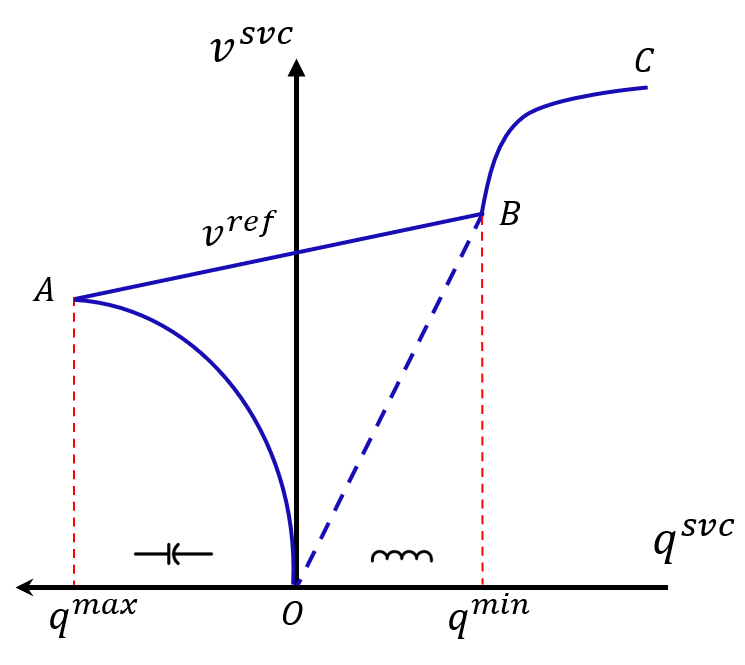
\includegraphics[width=\textwidth]{svc_linear_with_q.png}
		{\footnotesize (a) SVC linear with $Q$.}
	\end{minipage}
	\hfill
	\begin{minipage}{0.48\columnwidth}
		\centering
		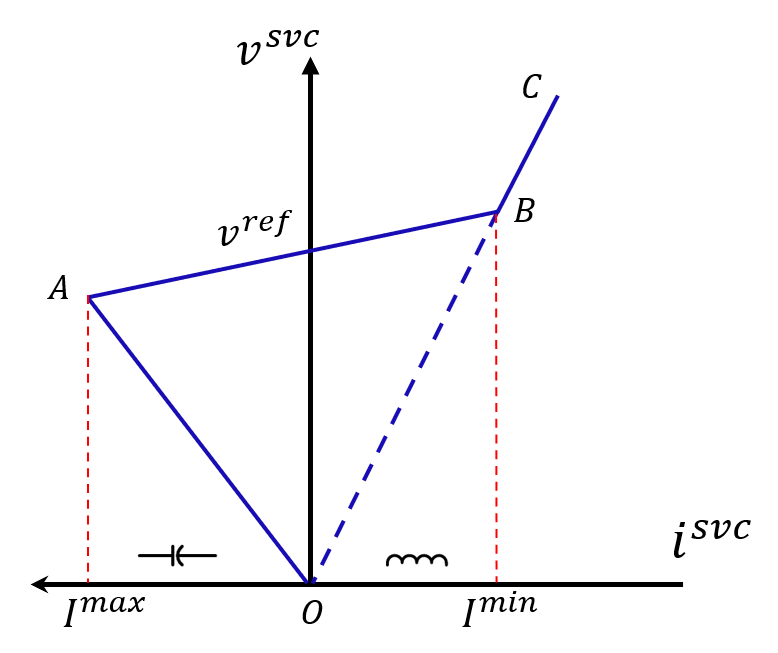
\includegraphics[width=\textwidth]{svc_linear_with_i.png}
		{\footnotesize (b) SVC linear with $I$.}
	\end{minipage}
	\caption{SVC control modes configurations.}
	\label{fig:svc_configurations}
\end{figure}
% ====================================================================================================================================
\subsection{Control Network Components}
\label{sec:controls}
% --- LTC ---
\subsubsection{On-load Tap Changers (LTC)}
For each LTC transformer $\ell \in \mathcal{L}_{\mathrm{ltc}}$ --- identified in the input data by a nonzero tap range and a
controlled bus --- the tap ratio $t_\ell$ is a continuous decision variable bounded by its mechanical limits:
\begin{equation}
	\label{eq:ltc_tap}
	t^{\min}_\ell \le t_\ell \le t^{\max}_\ell, \quad \forall \ell \in \mathcal{L}_{\mathrm{ltc}}.
\end{equation}
The tap enters the branch admittance terms of (\ref{eq:power_flow_3}) and (\ref{eq:power_flow_4}) through $1/t_\ell^{2}$ on the
self-side and $1/t_\ell$ on the mutual-side terms. The LTC regulates the voltage magnitude of its controlled bus toward the reference
value $v^{ref}_\ell$; because the tap is continuous in the NLP, the voltage target is enforced as a soft equation:
\begin{equation}
	\label{eq:ltc_control}
	v_{c\ell} - v^{ref}_\ell = r_\ell^{+} - r_\ell^{-}, \qquad r_\ell^{+} + r_\ell^{-} \le \varepsilon_{\mathrm{ctrl}},
	\quad \forall \ell \in \mathcal{L}_{\mathrm{ltc}},
\end{equation}
where $v_{c\ell}$ is the voltage magnitude of the controlled bus, $\varepsilon_{\mathrm{ctrl}}$ is the control tolerance, and the
residual slacks are penalized in the objective together with a small quadratic regularization $(t_\ell - t_\ell^{0})^2$ that keeps the
tap near the input setpoint. When tap optimization is disabled, $t_\ell$ is fixed at its input value and behaves as a parameter,
which matches the fixed-tap case.
% --- PST ---
\subsubsection{Phase-Shifting Transformers (PST)}
Phase-shifting transformers are represented by the fixed phase shift $\phi_\ell$ applied through the complex tap ratio in the
$\pi$-model; the trigonometric terms $\cos(\theta_{ij}+\phi_{ij})$ and $\sin(\theta_{ij}+\phi_{ij})$ in
(\ref{eq:power_flow_3}) and (\ref{eq:power_flow_4}) directly embed the PST action in the branch flows, without additional state
variables. The phase shift is read from the input data and kept fixed during the solution, which corresponds to a PST whose
setpoint is defined before solving the power flow.
% --- Switches ---
\subsubsection{Switches and Network Reduction}
Closed switches and electrically equivalent low-impedance breaker branches are contracted before the NLP is built. A switch or breaker
branch is contracted when it connects buses that remain at the same voltage profile, that is, when the branch is an exact switch, or
when its impedance is below the low-impedance threshold $Z_{\min}$ (default $0.001\%$) and the apparent flow through it exceeds
$125\%$ of its rating. The contraction merges the terminal buses with a union-find procedure: the generations, loads, and shunts of
all merged buses are aggregated at the representative bus (the one with the highest bus-type priority and external degree),
\begin{equation}
	\label{eq:switch_aggregation}
	P^{\mathrm{agg}}_i = \sum_{j \in \mathcal{M}_i} P^{\mathrm{orig}}_j, \qquad
	Q^{\mathrm{agg}}_i = \sum_{j \in \mathcal{M}_i} Q^{\mathrm{orig}}_j,
\end{equation}
where $\mathcal{M}_i$ is the set of original buses merged into the representative bus $i$, and the contracted branches are removed
from the network. A mapping back to the original buses is retained so that the solved voltages and control states are expanded to the
full, uncontracted topology for reporting. This step reduces the size of the NLP without changing the physics of the solved system.
% --- Switched shunts ---
\subsubsection{Switched Shunts}
Bus shunt banks with automatic switching are represented by a continuous control variable $q^{sh}_\ell$ for each controllable bank
$\ell \in \mathcal{Sh}$, bounded by the bank limits relative to its initial injection:
\begin{equation}
	\label{eq:shunt_var}
	q^{\mathrm{sh},\min}_\ell \le q^{sh}_\ell \le q^{\mathrm{sh},\max}_\ell,
	\quad \forall \ell \in \mathcal{Sh},
\end{equation}
and the bank injection $q^{sh}_\ell v_i^2$ enters the reactive balance of its bus through the aggregated term $Q_i^{sh}$ in
(\ref{eq:power_flow_2}). Fixed banks are treated as parameters and only contribute to $b_i^{sh}$. When the shunt voltage dead-band
is enforced, the controlled-bus voltage magnitude is constrained by the bank's operating limits:
\begin{equation}
	\label{eq:shunt_voltage}
	v^{\min}_\ell \le v_{c\ell} \le v^{\max}_\ell, \quad \forall \ell \in \mathcal{Sh},
\end{equation}
so that the model reproduces the automatic switching behavior of the banks through the continuous NLP solution.
% ====================================================================================================================================
% \vspace{-0.6cm}
\subsection{Line-Commutated Converter (LCC)}
 The steady-state modeling of LCC systems used in this work follows classical converter relationships, including converter-side voltages,
 current, control angles, and commutation effects. These relationships provide the analytical basis consistent with practical LCC rectifier
 and inverter operation used in AC/DC power flow studies.
The LCC system is modeled using a unified set of equations for both rectifier ($k=r$) and inverter ($k=i$) terminals \cite{ref15}. For each
pole $h \in \mathcal{H}$, where $\mathcal{H}$ represents the set of all active DC poles, the DC voltage $V^{dc,h}_k$ is expressed as the ideal
no-load voltage term plus the commutation reactance drop:
\begin{align}
	\label{eq:vdc_universal}
	V^{dc,h}_k = N^h_k \left(\frac{3 \sqrt{2}}{\pi}\frac{a^h_k V^{ac,h}_k}{T^h_k} \cos{\theta^h_k} + s_k\frac{3 X^{h}_k}{\pi} I^{dc,h}_k\right), \nonumber \\
	\forall h \in \mathcal{H}, \, k \in \{r,i\},
\end{align}
where $s_r=-1$ for the rectifier and $s_i=+1$ for the inverter, which physically accounts for the polarity change and internal voltage drop across
the bridges under commutation. The parameter $\theta^h_k$ denotes the operational control angle mapped to each terminal mode;
specifically, $\theta^h_r = \alpha^h_r$ represents the firing delay angle for the rectifier, whereas $\theta^h_i = \gamma^h_i$ represents
the minimum extinction angle for the inverter. Furthermore, $N^h_k$ is the number of bridges that the converter station possesses for pole $h$
at terminal $k$, $a^h_k$ is the transformer ratio, $T^h_k$ is the tap ratio, $X^h_k$ is the commutation reactance, and $I^{dc,h}_k$ is the DC
current flowing through the link.

The commutation process induces a phase displacement between the AC voltage and fundamental AC current. The corresponding overlap angle $\mu^h_k$
and power factor angle $\phi^h_k$ for each pole $h \in \mathcal{H}$ and terminal $k \in \{r,i\}$ are governed by:
\begin{align}
	\label{eq:overlap_angle_fix}
	\mu^h_k  & = \cos^{-1}\left(\cos\theta^h_k-\frac{\sqrt{2}\,I^{dc,h}_k X^{h}_k T^h_k}{a^h_k V^{ac,h}_k}\right)-\theta^h_k, \\
	\label{eq:phi_angle_fix}
	\phi^h_k & = \tan^{-1}\left(
	\frac{\sin(2\theta^h_k+2\mu^h_k)-\sin(2\theta^h_k)+2\mu^h_k}
	{\cos(2\theta^h_k)-\cos(2\theta^h_k+2\mu^h_k)}
	\right).
\end{align}
To guarantee mathematical and physical consistency within the NLP optimization framework, the argument of the inverse cosine in
\eqref{eq:overlap_angle_fix} is strictly constrained to the domain $[-1, 1]$, preventing non-convergence during high DC current or depressed
AC voltage states.

The \textit{RMS} AC current $I^{ac,h}_k$ at the converter transformer is proportional to the DC current, while the reactive power
variable $Q^{ac,h}_k$ at the AC interface is derived for all $h \in \mathcal{H}$ and $k \in \{r,i\}$ as follows:
\begin{align}
	I^{ac,h}_k & = \frac{\sqrt{6}}{\pi}N^h_k I^{dc,h}_k, \label{eq:iac_rms}                        \\
	Q^{ac,h}_k & = \sqrt{3}\, I^{ac,h}_k (a^h_k V^{ac,h}_k / T^h_k)\sin\phi^h_k. \label{eq:hvdc_q}
\end{align}
In the nodal balance, the active power terms $P^{ac,h}_{r}$ and $P^{ac,h}_{i}$ are treated as fixed setpoints specified by the system data models,
representing a withdrawal at the rectifier bus and an injection at the inverter bus, respectively. Conversely, because line-commutated converters
inherently consume reactive power regardless of power flow direction, both $Q^{ac,h}_{r}$ and $Q^{ac,h}_{i}$ are modeled strictly as reactive power
withdrawals. These variables are directly integrated into the nodal power balance equations \eqref{eq:power_flow_1} and \eqref{eq:power_flow_2}.
The two-terminal DC link closes its own circuit balance: one converter is designated as the slack (folga) terminal and fixes the DC voltage
of the pole, while the other terminal sets the transferred power (or current). The DC line resistance $R^{dc,h}$ allocates the losses and the
terminal voltage drop:
\begin{align}
	P^{dc,h}_{r} & = P^{dc,h}_{i} + (I^{dc,h})^2 R^{dc,h}, \label{eq:dc_power_balance} \\
	V^{dc,h}_{r} & = V^{dc,h}_{i} + I^{dc,h} R^{dc,h}.                    \label{eq:dc_voltage_drop}
\end{align}
Finally,
operational feasibility and equipment limits are enforced across all components by:
\begin{align}
	T^{\min,h}_k      & \leq T^h_k \leq T^{\max,h}_k, \quad \forall h \in \mathcal{H}, \, k\in\{r,i\}, \\
	\alpha^{\min,h}_r & \leq \alpha^h_r \leq \alpha^{\max,h}_r, \quad \forall h \in \mathcal{H},       \\
	\gamma^{\min,h}_i & \leq \gamma^h_i \leq \gamma^{\max,h}_i, \quad \forall h \in \mathcal{H}.
\end{align}
The converter transformer tap ratios $T^h_k$ are continuous variables that regulate the AC-side voltage seen by the bridges so that
$\alpha^h_r$ and $\gamma^h_i$ remain in secure operating ranges with controlled reactive demand.
% ====================================================================================================================================
\section{Simulation Process}

The model is implemented in Python/Pyomo and solved with Ipopt. The execution pipeline has four stages: (i) parsing and network reduction,
(ii) Newton--Raphson warm start, (iii) NLP build and solve, and (iv) post-solution restoration of control states for reporting.

The~.pwf file is first parsed and reduced by closed-switch/breaker contraction. Then, a Newton--Raphson solve provides a warm start for
Ipopt. The NLP of Section~\ref{sec:OB-ACPF} is solved from this seed, and solved control states are expanded back to the original
topology for reporting.

The model reads default values and execution options directly from the input records to reproduce Anarede behavior.
Table~\ref{tab:anarede_defaults} summarizes the numerical values used by the NLP and warm-start steps for tolerances,
iteration/step limits, and control activation options.

\begin{table}[htb]
	\centering
	\footnotesize
	\caption{Default constants and power-flow options used by the proposed model.}
	\label{tab:anarede_defaults}
	\renewcommand{\arraystretch}{1.2}
	\setlength{\tabcolsep}{2pt}
	\begin{tabular}{lll}
		\hline
		\textbf{Default} & \textbf{Description} & \textbf{Model usage}                  \\ \hline
		100 MVA  & Power base                  & Per-unit base of the model            \\
		0.1 MW   & Active balance tolerance    & Active balance tolerance              \\
		0.1 Mvar & Reactive balance tolerance  & Reactive balance tolerance            \\
		0.5\%    & Voltage control tolerance   & Control tolerance                     \\
		30       & Maximum iterations          & Solver iteration budget               \\
		40\%     & Minimum voltage divergence  & NR warm-start limit                   \\
		200\%    & Maximum voltage divergence  & NR warm-start limit                   \\
		0.05 rad & Maximum angle step          & NR step limit                         \\
		5\%      & Maximum voltage step        & NR step limit                         \\
		5\%      & Maximum CSC step            & NR step limit                         \\
		0.001\%  & Low-impedance threshold     & Switch/breaker contraction            \\
		option   & Reactive limits on PV buses & Q-limited PV variables                \\
		option   & LTC tap control             & LTC tap optimization                  \\
		option   & Shunt auto switching        & Switched-shunt variables              \\
		option   & PST phase-shift control     & PST setpoint read from data           \\ \hline
	\end{tabular}
\end{table}

\section{Numerical Results}
\label{sec:results}

\subsection{BIPS Data Model}

The study uses cases released by the Brazilian Independent System Operator~\cite{ref16}, grouped as equivalent planning models and
full operating snapshots. The planning set contains two 7k-bus models, while the 2024 snapshots contain 11,835 buses before
closed-switch contraction. An additional 247-bus equivalent case is used for detailed comparison against Anarede. Together, these
cases cover the main LCC corridors and representative FACTS controls of the BIPS.
TCSCs, SVCs, LTC transformers, PSTs, switched shunt banks, and bus and line capacitor/reactor banks.

As part of this study, the main LCC corridors currently relevant to BIPS operation are explicitly modeled. These include the Itaipu
link (Foz do Igua\c{c}u--Ibi\'una), the Madeira complex (Santo Ant\^onio--Araraquara, ABB and Areva bipoles), and the Belo Monte transmission
link (Xingu--Estreito and Xingu--Terminal Rio). In total, the implemented set comprises 12 poles organized as three major LCC schemes: four poles
at 600~kV for Foz/Ibi\'una, four poles at 600~kV for Santo Ant\^onio/Araraquara, and four poles at 800~kV for the Xingu corridors, with nominal pole
powers in the range of approximately 1566--2000~MW. Their representative operating settings are summarized in Table~\ref{tab:summary_lcc_links}.

\begin{table}[htb]
	\centering
	\footnotesize
	\caption{LCC line parameters in the BIPS.}
	\label{tab:summary_lcc_links}
	\renewcommand{\arraystretch}{1.2}
	\setlength{\tabcolsep}{6pt}
	\begin{tabular}{ccccc}
		\hline
		\textbf{\begin{tabular}[c]{@{}c@{}}Line\\ Name\end{tabular}}    &
		\textbf{\begin{tabular}[c]{@{}c@{}}Voltage\\ (kV)\end{tabular}} &
		\textbf{\begin{tabular}[c]{@{}c@{}}Power\\ (MW)\end{tabular}}   &
		\textbf{\begin{tabular}[c]{@{}c@{}}Pole\\ No.\end{tabular}}     &
		\textbf{$\alpha / \gamma$ ($^\circ$)}                                                                 \\ \hline
		Itaipu                                                          & 600/587.7 & 1050/1018 & 4 & 15/17   \\ \hline
		Madeira 1                                                       & 600/557.2 & 1500/1393 & 2 & 15/17   \\
		Madeira 2                                                       & 600/560.4 & 1500/1401 & 2 & 13/18   \\ \hline
		Belo Monte 1                                                    & 800/765.2 & 2000/1913 & 2 & 14.3/15 \\
		Belo Monte 2                                                    & 800/759.5 & 2000/1899 & 2 & 18.4/17 \\ \hline
	\end{tabular}
\end{table}

\subsection{Model Validation}
Validation is performed on equivalent and full BIPS cases with LCC links from Table~\ref{tab:summary_lcc_links}. For the equivalent case,
the AC side starts from a flat profile and one converter terminal per link keeps DC voltage reference. The proposed model reproduces the
operational trends observed in Anarede for voltages, angles, generator outputs, branch flows, and control setpoints. To make this
comparison explicit, Figs.~\ref{fig:equivalent_bips_model_ac_components} and \ref{fig:equivalent_bips_model_dc_components}
show the equivalent-case AC and DC validation results, respectively.

\begin{figure}[!htbp]
	\centering
	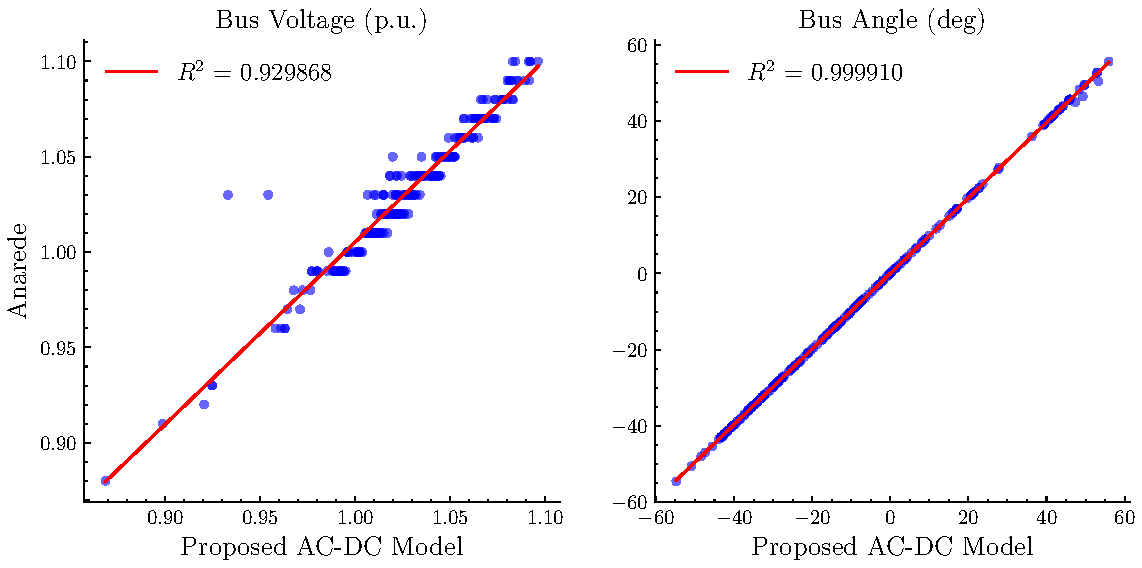
\includegraphics[width=0.95\columnwidth]{LENA_CASO_FINAL_EQV2020_DC_Full_bus_voltage_angle_results.pdf} \\[0.3em]
	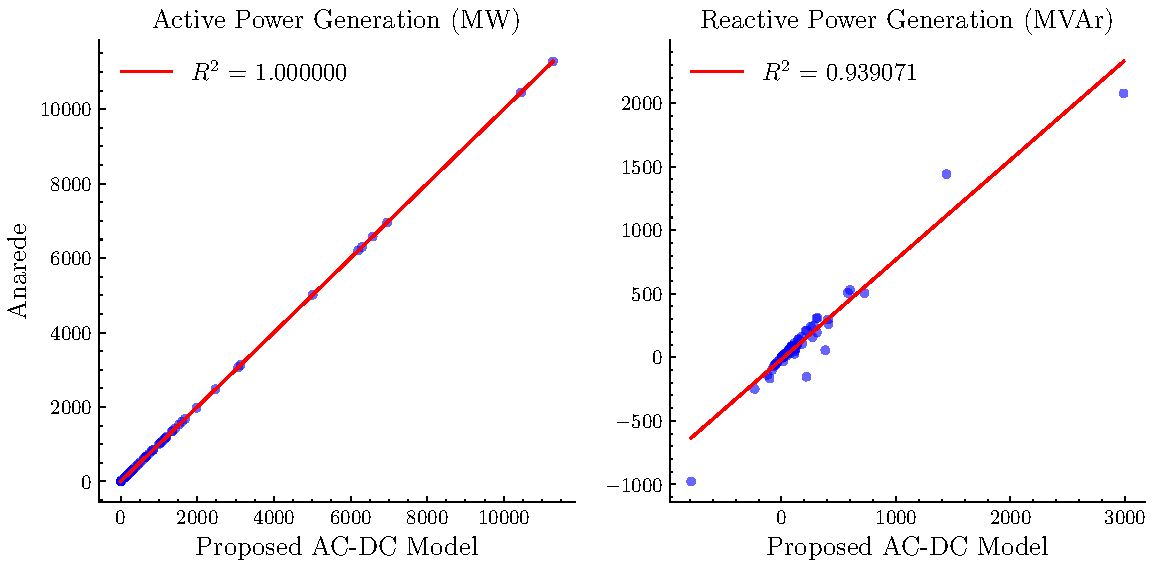
\includegraphics[width=0.95\columnwidth]{LENA_CASO_FINAL_EQV2020_DC_Full_generation_active_reactive.pdf} \\[0.3em]
	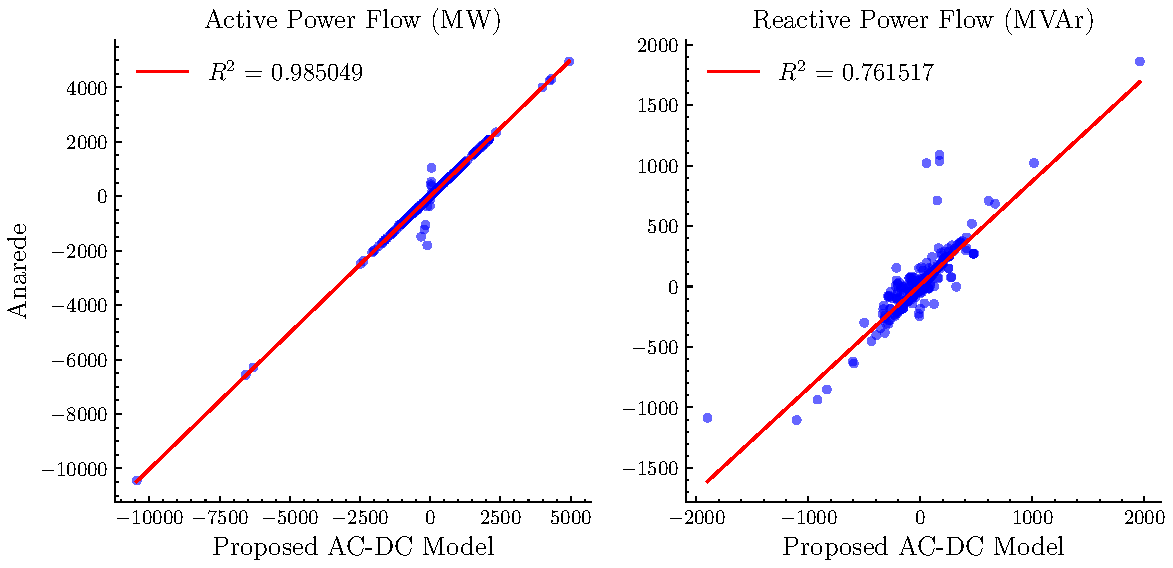
\includegraphics[width=0.95\columnwidth]{LENA_CASO_FINAL_EQV2020_DC_Full_branch_flow_active_reactive.pdf} \\[0.3em]
	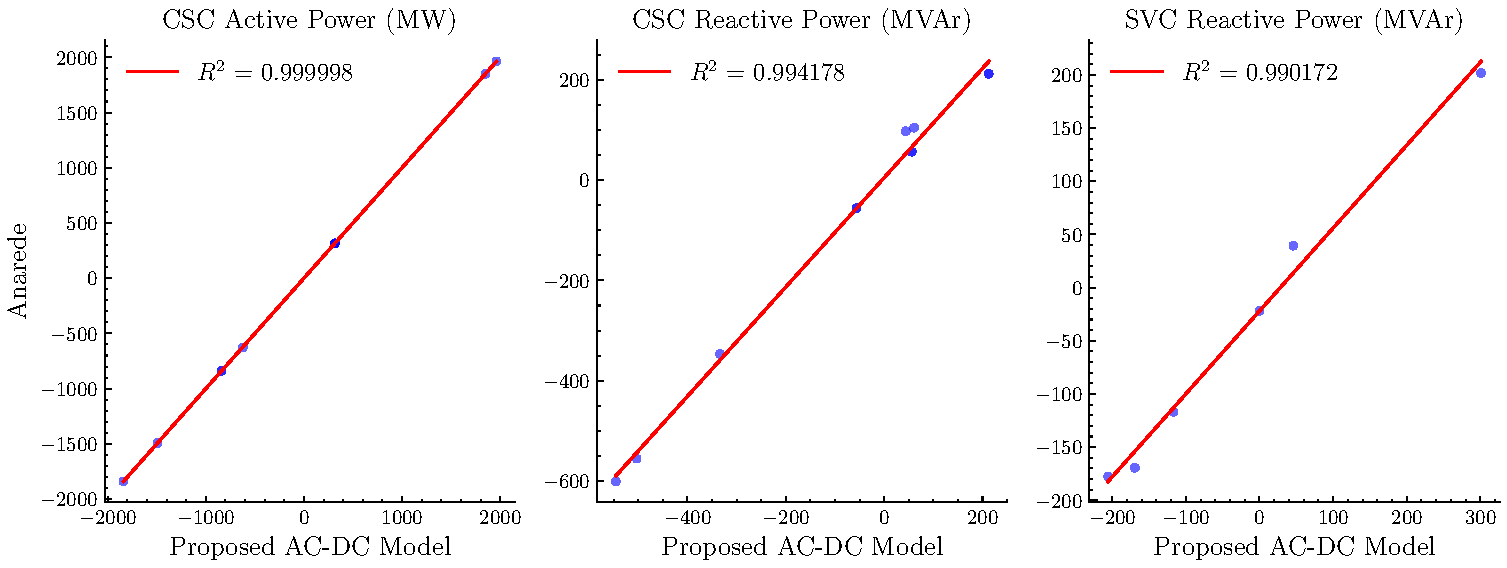
\includegraphics[width=0.95\columnwidth]{LENA_CASO_FINAL_EQV2020_DC_Full_csc_svc_results.pdf}
	\caption{Equivalent-case comparison against Anarede for AC variables: bus voltages/angles, generation, branch flows, and FACTS outputs.}
	\label{fig:equivalent_bips_model_ac_components}
\end{figure}

\begin{figure}[!htbp]
	\centering
	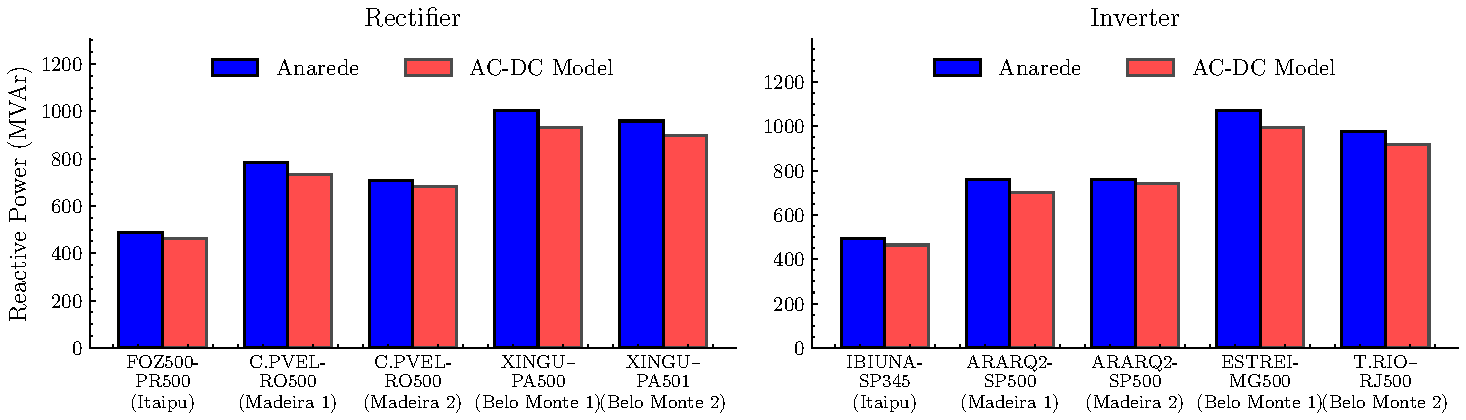
\includegraphics[width=0.95\columnwidth]{LENA_CASO_FINAL_EQV2020_DC_Full_hvdc_reactive_power.pdf} \\[0.5em]
	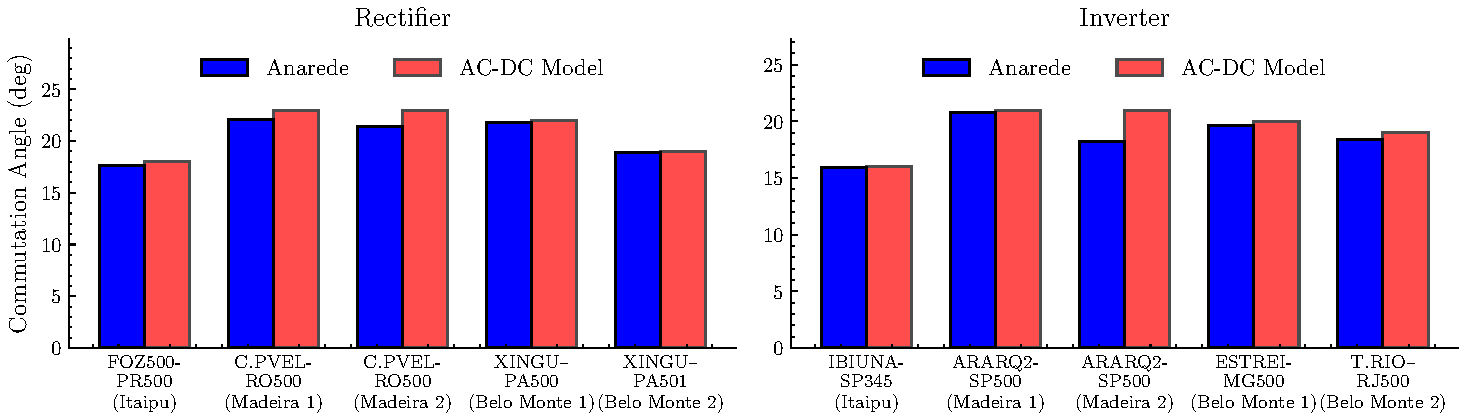
\includegraphics[width=0.95\columnwidth]{LENA_CASO_FINAL_EQV2020_DC_Full_hvdc_commutation_angle.pdf} \\[0.5em]
	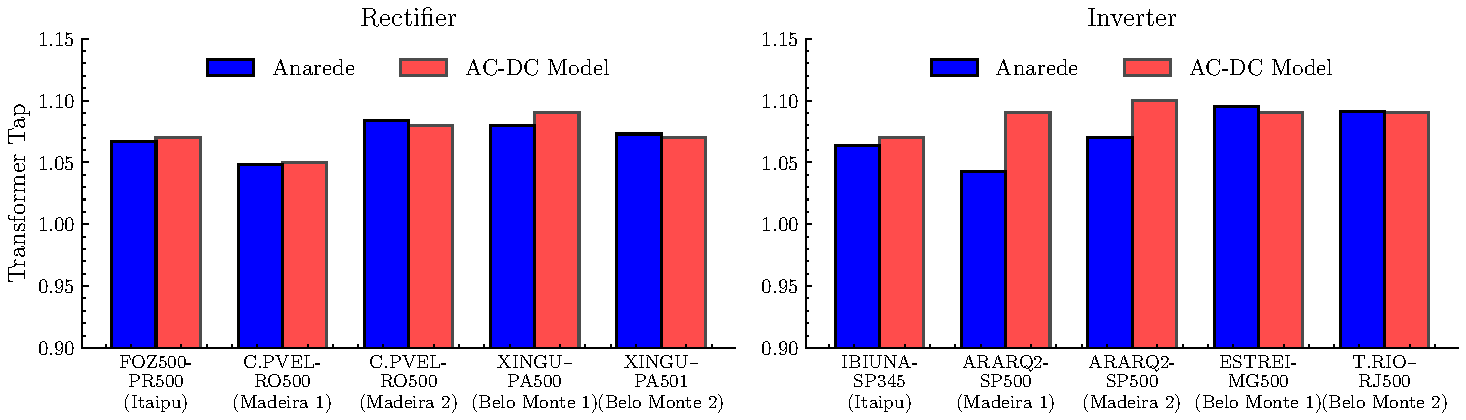
\includegraphics[width=0.95\columnwidth]{LENA_CASO_FINAL_EQV2020_DC_Full_hvdc_transformer_tap.pdf}
	\caption{Equivalent-case comparison against Anarede for LCC variables: converter reactive power, commutation angles, and tap ratios.}
	\label{fig:equivalent_bips_model_dc_components}
\end{figure}

Differences are mainly associated with alternative modeling assumptions and the existence of multiple feasible local solutions in large NLPs.
The Newton--Raphson warm start keeps the final solution near the input operating point, while optimization enforces feasible converter control,
including firing/extinction angles in practical ranges.

\begin{figure}[!htbp]
	\centering
	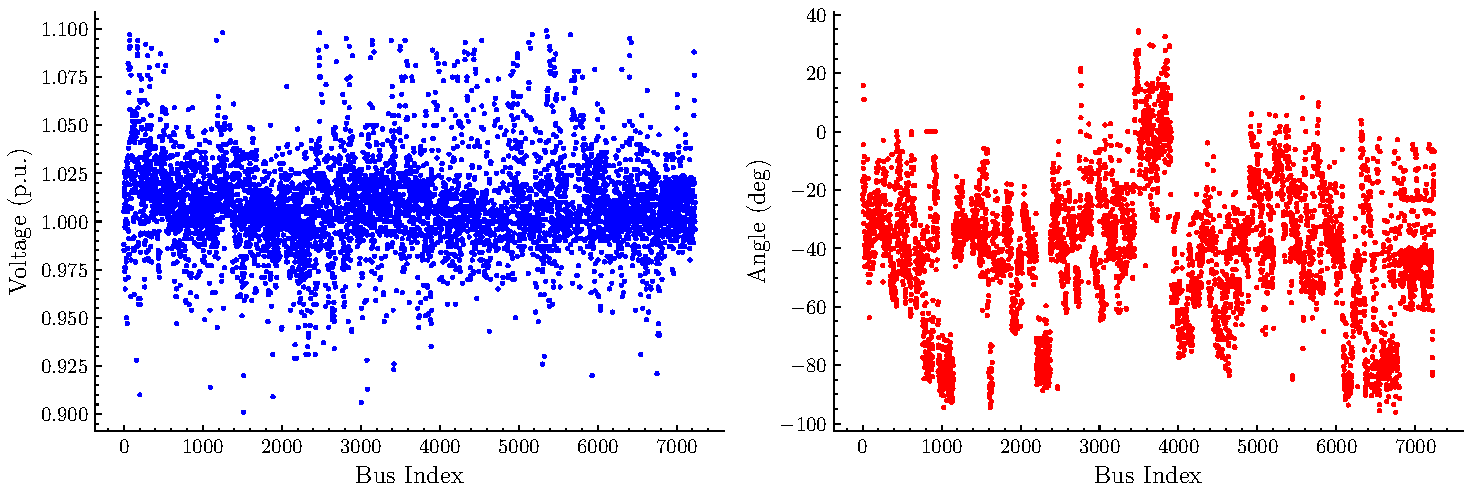
\includegraphics[width=0.95\columnwidth]{LEN_A_4_2020_SECO_2023VM_SE_EXP_N_4DC_bus_voltage_angle.pdf} \\[0.5em]
	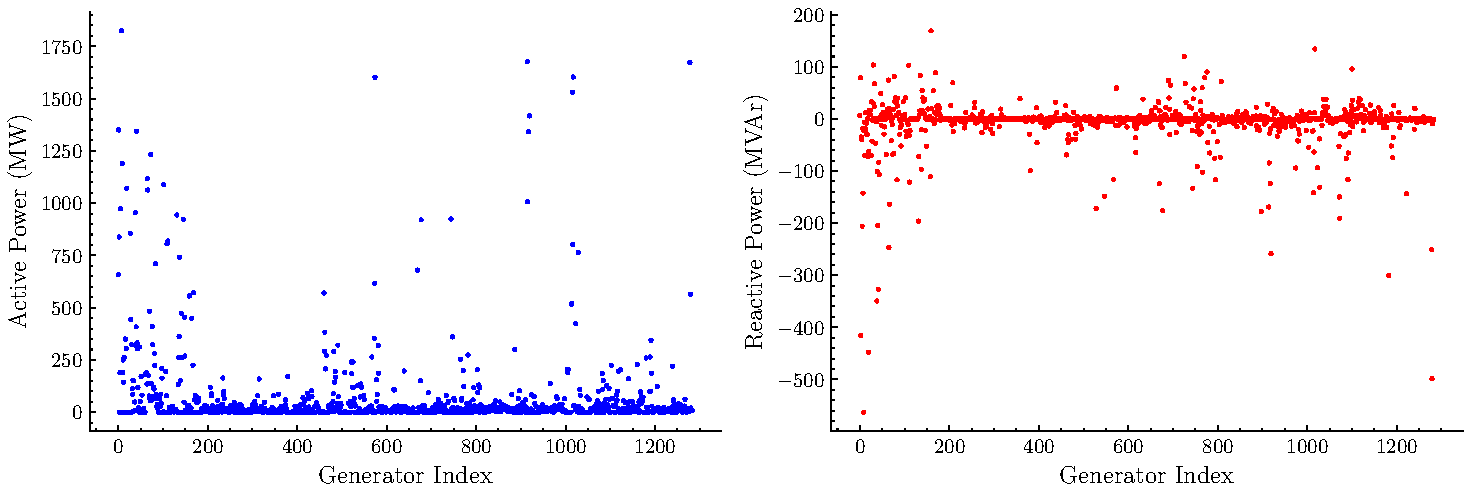
\includegraphics[width=0.95\columnwidth]{LEN_A_4_2020_SECO_2023VM_SE_EXP_N_4DC_generation_scatter.pdf}
	\caption{Large-scale comparison against Anarede for bus states and generator dispatch.}
	\label{fig:bus_validation}
\end{figure}

For large-scale snapshots, bus and generation profiles remain inside operational ranges and support the expected stressed-transfer behavior.
Transformer taps and converter controls stay within limits, and FACTS/LCC formulations maintain feasible operation without discrete switching.

\subsection{Convergence and Performance}
\label{sec:convergence}
This section reports convergence on all analyzed cases using the full optimization-based workflow.
Each run contracts closed switches, warm-starts with Newton--Raphson, and solves the NLP with Ipopt under the squared-generation
objective (Section~\ref{sec:OB-ACPF}). Table~\ref{tab:case_summary} summarizes the system data of each case, reporting the number of buses in the
full parsed case (the \texttt{DBAR} block, before the network reduction) and in the reduced case that the NLP is actually solved on, together
with the total active and reactive generation and load ($P_g, Q_g, P_l, Q_l$) computed from the per-bus values of the full case.

\begin{table}[!htbp]
	\centering
	\scriptsize
	\caption{Summary of the analyzed BIPS power flow cases}
	\label{tab:case_summary}
	\renewcommand{\arraystretch}{1.2}
	\setlength{\tabcolsep}{4pt}
	\begin{adjustbox}{width=\columnwidth}
	\begin{tabular}{lccccc}
		\hline
		\textbf{Case} & \textbf{Buses} & \textbf{$P_g$ (MW)} & \textbf{$P_l$ (MW)} & \textbf{iter} & \textbf{time (s)}\\ \hline
		\texttt{EQV-BIPS1}     & 247 & 85\,231     & 109\,228 & 17 & 2 \\
		\texttt{EQV-BIPS2}     & 7\,282 & 107\,532 & 125\,232 & 25 & 37 \\
		\texttt{BIPS 00-00}  & 11\,835 & 70\,310  & 74\,843 & 58 &  70 \\
		\texttt{BIPS 06-30}  & 11\,835 & 84\,088  & 73\,292 & 83 & 120 \\ \hline
	\end{tabular}
	\end{adjustbox}

	% \footnotesize
	% \texttt{LENA} = \texttt{LEN\_A\_4\_2020\_SECO\_2023VM\_SE\_EXP\_N}, \texttt{LENABD} = \texttt{LENA\_BD0320R0\_2Q2020\_R1\_CASO\_12},
	% \texttt{C 00-00}/\texttt{C 00-30}/\texttt{C 06-30} = \texttt{20240820\_C\_00-00}/\texttt{\_00-30}/\texttt{\_06-30.pwf},
	% \texttt{CASO} = \texttt{CASO\_FINAL\_EQV2020.pwf}.
\end{table}

All cases in Table~\ref{tab:case_summary} converged to an \texttt{optimal} Ipopt solution under the squared-generation objective,
with exact AC power-balance equations and bounded controller residuals. The equivalent cases converge quickly, while the 2024 full
snapshots are computationally dominated by the Newton--Raphson warm start due to size and operating stress. Even so, all snapshots
reach feasible, physically consistent operating points without retuning model weights.

% ===========================================================================================
\section{Conclusions}

This paper presented an open-source optimization-based integrated AC/DC power flow model for large-scale BIPS studies with detailed
LCC and FACTS representations. The formulation converged to feasible \texttt{optimal} solutions on equivalent and full-scale cases,
including 2024 operating snapshots, while maintaining numerically consistent trends against Anarede. These results indicate that the
proposed model is a practical basis for large-system AC/DC analysis. As future work, additional strategies to reduce iteration count
and total solve time will be investigated.

% ==============================================================================================================
\begingroup
\hbadness=10000
\begin{thebibliography}{1}
	\bibliographystyle{IEEEtran}


	\bibitem{ref1}
	B. Stott, "Review of load-flow calculation methods". In Proceedings of the IEEE, vol. 62, no. 7, pp. 916-929, July 1974, doi: 10.1109/PROC.1974.9544.

	\bibitem{ref2}
	E. H. Watanabe, P. G. Barbosa, K. C. Almeida, and G. N. Taranto, "Tecnologia FACTS - Tutorial". \textit{SBA Controle \& Automação}, vol. 9, no. 1, pp. 1--15, 1998.

	\bibitem{ref3}
	J. Beerten, S. Cole, and R. Belmans, “Generalized steady-state VSC MTDC model for sequential AC/DC power flow algorithms,” IEEE Trans. Power Syst., vol. 27, no. 2, pp. 821–829, May.
	2012.

	\bibitem{ref4}
	J. Beerten and R. Belmans, "Development of an open source power flow software for high voltage direct current grids and hybrid ac/dc systems: MatACDC". IET Gener. Transm. Distrib., vol. 9, no. 10, pp. 966–974, 2015.

	\bibitem{ref5}
	J. Lei, T. An, Z. Du, and Z. Yuan. "A general unified ac/dc power flow algorithm with MTDC". IEEE Trans. on Power Syst., vol. 32, no. 4, pp. 2837–2846, 2016.

	\bibitem{ref6}
	E. Acha, C. R. Fuerte-Esquivel, H. Ambriz-P\'erez, and C. Angeles-Camacho, "FACTS: Modeling and Simulation in Power Networks". Chichester, U.K.: John Wiley \& Sons, 2004, doi: 10.1002/0470020164.

	\bibitem{ref7}
	W. A. Bukhsh, "On Solving the Load Flow Problem as an Optimization Problem". Univ. Strathclyde, Glasgow, U.K., Tech. Rep., 2018. [Online]. Available: https://pure.strath.ac.uk

	\bibitem{ref8}
	A. Wächter and L. T. Biegler, "On the Implementation of a Primal-Dual Interior Point Filter Line Search Algorithm for Large-Scale Nonlinear Programming". \textit{Math. Program.}, vol. 106, no. 1, pp. 25--57, 2006.

	\bibitem{ref9}
	CEPEL, DRE, "Network Analysis Program (ANAREDE), Version 10.01.00: User Manual", Centro de Pesquisas de Energia El\'etrica, Rio de Janeiro, Brazil, Sep. 2015. [Online]. Available: http://www.cepel.br

	\bibitem{ref10}
	L. Braz, C. Castro, and C. Murati, "A critical evaluation of step size optimization based load flow methods", IEEE Transactions on Power Systems, vol. 15, no. 1, pp. 202–207, 2000.

	\bibitem{ref11}
	C. Coffrin, R. Bent, K. Sundar, Y. Ng, and M. Lubin, "PowerModels.jl: An Open-Source Framework for Exploring Power Flow Formulations," in \textit{2018 Power Systems Computation Conference (PSCC)}, Dublin, Ireland, 2018, pp. 1--8, doi: 10.23919/PSCC.2018.8442948.

	\bibitem{ref12}
	Padiyar, K.R, "FACTS Controllers in Power Transmission and Distribution". New Age International Pvt. Limited, New Delhi. 2027.

	\bibitem{ref13}
	J. Arrillaga, "High Voltage Direct Current Transmission", 2nd ed. London, U.K.: The Institution of Engineering and Technology, 2008.

	\bibitem{ref14}
	J. Arrillaga and B. Smith, "AC-DC Power System Analysis". London, U.K.: The Institution of Electrical Engineers, 1998.

	\bibitem{ref15}
	PTI, Inc., "PSS\textsuperscript{\textregistered}E 34.9.5 Program Application Guide, Volume 1". Schenectady, NY, USA: Siemens Power Technologies International, May 2022.

	\bibitem{ref16}
	Operador Nacional do Sistema Elétrico (ONS), "ONS (Operador Nacional do Sistema Elétrico)", 2025. [Online]. Available: https://www.ons.org.br/. Accessed: Apr. 20, 2025.

\end{thebibliography}
\endgroup

\end{document}